\subsubsection*{Le matin :}
Des graphiques ont étés générés a partir des données :

\begin{figure}[H]
    \center
    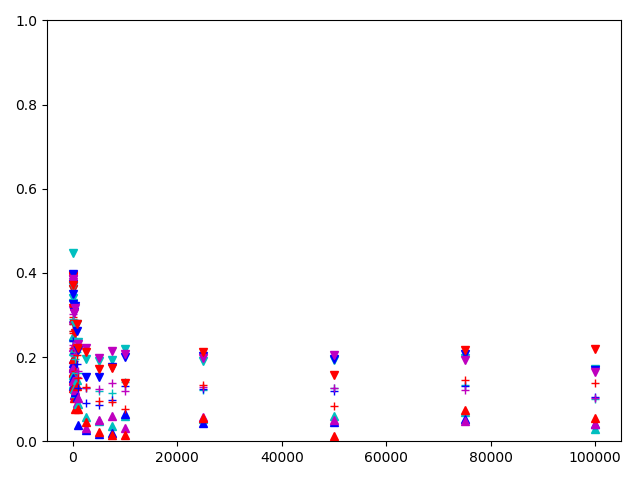
\includegraphics[height=\petit]{sources/data/etfdata/graph3.png}
    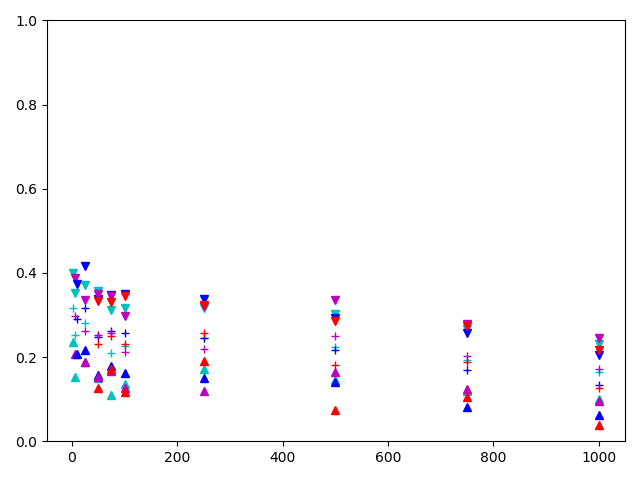
\includegraphics[height=\petit]{sources/data/etfdata/graph4.png}
	\caption{Ecart type de l'apprentissage en fonction de la taille de la base de données}
	\label{etfdata2graph}
\end{figure}
\vspace{-5pt}
On peut voir ici que l'erreur d'aprentissage s'amoindrit avec l'augmentation de la taille du learning set.
Cette évolution s'arette vers les $1000$ données, dépassé ce cap, l'écart type stagne.


\subsubsection*{L'après midi :}
Tout un module a été codé afin de visualiser les données.
Une variante des premiers graphiques a été réalisé :
Un graphique a taille de base de donnée fixée de l'écart type de l'apprentissage en fonction du nombre d'aprensitssages réalisés par le réseau.
Cette technique permet de s'afranchir du problème posé le 16 mai en ne stagnant pas dans un minimum local.

\begin{figure}[H]
    \center
    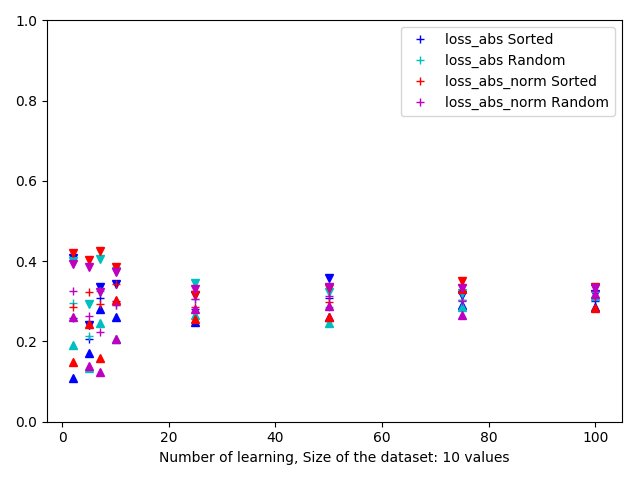
\includegraphics[height=\moyen]{sources/data/etfn/graph1.png}
	\caption{Ecart type de l'apprentissage moyen en fonction du nombre d'aprensitssages}
	\label{etfngraph1}
\end{figure}
\vspace{-5pt}
Ici on peut voir que la moyenne ne varie pas significativement mais l'ecart type diminue drastiquement.
Ce parametre combiné au precedent permetra d'augmenter la précision du réseau.
